% ------------------------------------------------------------------------
% ------------------------------------------------------------------------
% abnTeX2: Modelo de Trabalho Acadêmico (tese de doutorado, dissertação de
% mestrado e trabalhos monográficos em geral) em conformidade com
% as normas da ABNT
% ------------------------------------------------------------------------
% ------------------------------------------------------------------------

\documentclass[english, 
               brazil, 
               msc] %Opções msc (Mestrado)
               {ppgpi-abntex2}
% Geração de dummy text
% Retirar para a versão final do documento


%Compila o indíce
\makeindex

\begin{document}

% Seleciona o idioma do documento (conforme pacotes do babel)
\selectlanguage{brazil}

% Retira espaço extra obsoleto entre as frases.
\frenchspacing 

% ----------------------------------------------------------
% ELEMENTOS PRÉ-TEXTUAIS
% ----------------------------------------------------------

\pretextual


\titulo{Programa Empreenda AGRO Sustentável como mecanismo indutor de inovação}
\orientador{Prof. Dr. }
\author{Luiz Diego Vidal Santos}


\curso{Ciência da Propriedade Intelectual}

\imprimircapa

\imprimirfolhaderosto

%\imprimirfichacatalografica
%\imprimirfolhadeaprovacao
%\begin{dedicatoria}
   \vspace*{\fill}
   \centering
   \noindent
   \textit{Dedico essa dissertação aos meus pais, que me permitiram criar peças e não apenas apertar parafusos.} \vspace*{\fill}
\end{dedicatoria}
% ---
%\begin{agradecimentos}

A minha família pelo apoio, colaboração, amor, empenho e paciência. 

A minha noiva pelo apoio nos momentos difíceis e de vontade de desistência, me guiando para o melhor caminho.

Ao meu orientador pela oportunidade de me expressar inventivamente, me apoiar durante todo o projeto assim como orientar nos desvarios que surgiram no meio do caminho.

Aos colegas de curso pela amizade, companheirismo, espontaneidade e alegria ao longo desses anos de convivência.

E, finalmente, a Deus pela fé e força depositadas em mim para que eu pudesse enfrentar este curso e conseguir concluí-lo.
\end{agradecimentos}
% ---
%\begin{epigrafe}[]
    \vspace*{\fill}
	\begin{flushright}
	
		\textit{"A plenitude da atividade humana é alcançada somente quando nela coincidem, se acumulam,\\ se exaltam e se mesclam o trabalho o estudo e o jogo; isto é,  quando nós \\ trabalhamos, aprendemos e nos divertimos, tudo ao mesmo tempo."\\
				\textbf{Domenico de Masi}}
		
	\end{flushright}
\end{epigrafe}
% ---

, ,  

% % resumo em português
\setlength{\absparsep}{18pt} % ajusta o espaçamento dos parágrafos do resumo
\begin{resumo}

Ser empreendedor não significa apenas ter seu próprio negócio, o empreendedorismo está ligado às ações e capacidades individuais para criar, modular e sustentar ideias inovadoras globalmente. Assim, as ideias normalmente estão ligadas à inovação, algo que transcende o comum. Algumas ferramentas tais como workshops, jornadas, cursos, palestras podem ser usadas para difusão do comportamento empreendedor tanto em órgãos privados como em instituições de ensino, de modo a incutir novas ações empreendedoras sustentáveis, no sentido comercial, nas áreas industriais e agrícolas no meio acadêmico. Faz-se necessário, então, a construção de um cenário favorável ao desenvolvimento da cultura empreendedora no ambiente acadêmico, principalmente nas ciências agrárias. Neste contexto, muitas nações estão buscando promover atividades empreendedoras, utilizando, para isto, programas educacionais promovidos nos meios acadêmicos alcançando um importante público jovem. Neste sentido, este estudo tem como objetivo identificar, de forma analítica, a inovação sustentável e a eficácia do incentivo ao empreendedorismo por meio de uma ação educacional com vistas aos negócios rurais, tendo como ferramenta promotora o Programa Empreenda AGRO Sustentável. O Programa visa buscar o engajamento dos alunos para o desenvolvimento de novos negócios direcionados ao setor agrícola, podendo este experimento também direcionar futuras pesquisas científicas focadas em produtos capazes de satisfazer às novas demandas, de forma eficiente e sustentável. A metodologia de natureza quantitativa exploratória e de estudo de caso foi utilizada para avaliar quantitativamente o Programa Empreenda AGRO Sustentável com coleta de dados por meio da técnica “survey” tendo como base o estudo GUESS. A ferramenta de promoção prática do comportamento empreendedor “Programa Empreenda AGRO Sustentável" foi conduzida buscando a disseminação do empreendedorismo junto aos acadêmicos do Centro de Ciências Agrárias Aplicadas da Universidade Federal de Sergipe (UFS). Quatro Workshops foram planejados e executados de maneira sistemática e interativa, em que foram aplicadas metodologias e ferramentas para modelagem de negócios como Design Thinking com o intuito de despertar ideias de startups por meio de oficinas interdisciplinares fomentando, desta forma, a construção de Mínimos Produtos Comercialmente Viáveis (MCVP). Por meio do Programa Empreenda Agro Sustentável e a partir da aplicação das metodologias ativas, 15 equipes discutiram e amadureceram ideias em modelos de startups, resultando em modelos de negócios escaláveis e negociáveis direcionados ao meio rural. Como resultado, a pesquisa constatou que os alunos participantes apresentaram forte influência positiva na intenção empreendedora e na autoeficácia para o empreendedorismo. Além disso, a pesquisa demonstrou que os alunos envolvidos no decorrer do programa evoluíram positivamente as dimensões empreendedoras estudadas, influenciando assim o desenvolvimento de novos negócios planejados na etapa de pré-aceleração, e encontraram maior segurança para o próximo passo que é o de aceleração de seus planos de negócios, conquistando autonomia, buscando novas oportunidades como profissionais proativos no mercado de trabalho.

\textbf{Palavras-chave}: Comercialização; Negócios sustentáveis; Propriedade Intelectual; Desenvolvimento rural.
\end{resumo}


% resumo em inglês
\setlength{\absparsep}{18pt} % ajusta o espaçamento dos parágrafos do resumo
\begin{resumo}[Abstract]
 \begin{otherlanguage*}{english}
   
Being an entrepreneur does not just mean having your own business, entrepreneurship is linked to individual actions and capabilities to create, modulate and sustain innovative ideas globally. Thus, ideas are usually linked to innovation, something that transcends the ordinary. Some tools such as workshops, seminars, courses, lectures can be used to disseminate entrepreneurial behavior both in private bodies and in educational institutions, in order to instill new sustainable entrepreneurial actions, in the commercial sense, in the industrial and agricultural areas in the academic environment. . It is necessary, then, to build a favorable scenario for the development of entrepreneurial culture in the academic environment, mainly in the agricultural sciences. In this context, many nations are seeking to promote entrepreneurial activities, using educational programs promoted in academic circles to reach an important young audience. In this sense, this study aims to identify, in an analytical way, sustainable innovation and the effectiveness of encouraging entrepreneurship through an educational action aimed at rural businesses, using the Empreenda AGRO Sustentável Program as a promoting tool. The Program aims to seek student engagement for the development of new businesses aimed at the agricultural sector, and this experiment can also direct future scientific research focused on products capable of satisfying new demands, in an efficient and sustainable manner. The methodology of quantitative exploratory nature and case study was used to quantitatively evaluate the Empreenda AGRO Sustentável Program with data collection using the “survey” technique based on the GUESS study. The tool for the practical promotion of entrepreneurial behavior “Programa Empreenda AGRO Sustentável” was conducted seeking the dissemination of entrepreneurship among academics at the Center for Applied Agricultural Sciences at the Federal University of Sergipe (UFS). Four workshops were planned and executed in a systematic and interactive way , in which methodologies and tools for business modeling such as Design Thinking were applied in order to awaken ideas from startups through interdisciplinary workshops, thus promoting the construction of Minimum Commercially Viable Products (MCVP). Sustainable and based on the application of active methodologies, 15 teams discussed and matured ideas in models of startups, resulting in scalable and negotiable business models aimed at the rural environment. As a result, the research found that the participating students had a strong positive influence on the intention entrepreneur a and self-efficacy for entrepreneurship. In addition, the research demonstrated that the students involved in the course of the program positively evolved the entrepreneurial dimensions studied, thus influencing the development of new businesses planned in the pre-acceleration stage, and found greater security for the next step, which is the acceleration of their business plans, gaining autonomy, seeking new opportunities as proactive professionals in the job market.

 \textbf{Keywords}:Sustainable business, Intellectual Property, Extension Project.
 \end{otherlanguage*}
\end{resumo}
    
 %Lista de Figuras %%%%%%%%%%%%%%
    \pdfbookmark[0]{\listfigurename}{lof}
     \listoffigures*
   \cleardoublepage

% Lista de Tabelas %%%%%%%%%%%%%
    \pdfbookmark[0]{\listtablename}{lot}
     \listoftables*
    \cleardoublepage

\cleardoublepage
   
% ---
% inserir lista de abreviaturas e siglas
% ---

\begin{siglas}
%\item[ABP]{ Aprendizagem Baseada em Problemas}
%\item[CCAA]{Centro de Ciências Agrárias Aplicadas}
\item[DPI]{Direito de Propriedade Intelectual}
%\item[EE]{Educação Empreendedora}
%\item[EAESP]{Escola de Administração de Empresas de São Paulo}
%\item[FGV]{Fundação Getúlio Vargas}
%\item[GUESSS]{\textit{Global University Entrepreneurial Spirit Students Survey}}
\item[INPI]{Instituto Nacional da Propriedade Intelectual}
%\item[KMO]{Kaiser-Meyer-Olkin}
%\item[K-S]{Kolmogorov-Smirnov}
%\item[MCVP]{Mínimo Produto Comercialmente Viável}
%\item[OMPI]{Organização Mundial da Propriedade Intelectual}
\item[PI]{Propriedade Intelectual}
\item[TT]{Transferência de Tecnologia}
\item[UFS]{Universidade Federal de Sergipe}
\end{siglas}
% ---
%% ---
% inserir lista de símbolos
% ---

\begin{simbolos}
  \item[$ \sum  $] Letra grega Sigma
  \item[$ \int $] Integral
  \item[$ \omega $] Letra grega ómega
\end{simbolos}
% ---
\pdfbookmark[0]{\contentsname}{toc}
\tableofcontents*
\cleardoublepage

% ----------------------------------------------------------
% ELEMENTOS TEXTUAIS
% ----------------------------------------------------------
\textual
\chapter{INTRODUÇÃO}



\section{JUSTIFICATIVA}

Esta pesquisa está focada na dissonância entre a teoria e prática dos métodos educacionais e as grandes e contínuas mudanças do mercado de trabalho no meio rural. Este setor foi escolhido por estar contribuindo significativamente para a balança comercial do país, apresentando saldos positivos frequentes. Igualmente contribui para a segurança alimentar do País e produção de produtos limpos e renováveis. O mercado emergente apresenta significativa contribuição para a empregabilidade da população no campo, invertendo cada vez mais o êxodo rural, porém, este mercado que absorve novos profissionais, exige que tais profissionais sejam capazes de lidar com o desenvolvimento tecnológico e a produção em larga escala. 

\section{OBJETIVOS}

\subsection{OBJETIVO GERAL}


\subsection{OBJETIVOS ESPECÍFICOS}

\begin{itemize}
\item{;}
\item {;}
\item {;}
\item {}
\end{itemize}

\section{PROBLEMA}


\section{HIPÓTESE}




%%%%%%%%%%%%%%%%%%%%%%%%%%%%%%%%%%%%%%%%%%%%%%%%%%%%%%%%%%%%%%%%%%%%%%%%%%%%%%%%%%%%%%%%%%%%%%%%%%%%%%%%%%%%%%%%%%%%%%%%%%%%%%%%%%%%%%%%%%%%%%%%%%%%%%
                                                                 %REFERENCIAL TEÓRICO%                                                                             
%%%%%%%%%%%%%%%%%%%%%%%%%%%%%%%%%%%%%%%%%%%%%%%%%%%%%%%%%%%%%%%%%%%%%%%%%%%%%%%%%%%%%%%%%%%%%%%%%%%%%%%%%%%%%%%%%%%%%%%%%%%%%%%%%%%%%%%%%%%%%%%%%%%%%%
\chapter{REFERENCIAL TEÓRICO}


\section{Inovação para o desenvolvimento rural}

O empreendedorismo quando relacionado à inventividade não consiste apenas na criação de uma empresa. Ser empreendedor vai além de ter seu próprio negócio e implica em uma visão de mundo diferente, uma mudança de paradigma, de pensamento. Garcia \cite{garcia_formacao_2000} define o empreendedorismo inovativo como sendo a habilidade de criar e de construir algo a partir do nada, sendo, desta forma, um ato humano nascido da criatividade. O empreendedor é um constante inovador, sendo aquele que está sempre em busca de soluções, que consegue enxergar nas oportunidades, tendo iniciativa e sendo proativo e visionário. Dessa forma, podendo contribuir para introduzir inovações na empresa na qual trabalha, ajudar a solucionar problemas da sua cidade, entre outras possibilidades que se fazem presentes a partir do momento que um comportamento empreendedor é desenvolvido, \cite{alencar_intencao_2019, loiola_cao_2016}.

A inovação, a propagação da inovação e o surgimento de novos empreendimentos, em muitos países, são importantes sinais para o crescimento e recuperação de crises econômicas \cite{silva_educacao_2017}. A inovação é orientada de acordo com várias racionalidades, podendo ser observada por diversas óticas e utilizando diversos instrumentos para aprendizado \cite{munoz_innovacion_2016}. Com efeito, o ambiente acadêmico se apresenta como uma unidade básica para o desenvolvimento de novos processos inovadores onde tais conteúdos devem ser amplamente explorados \cite{costa_inovacao_2017}. 

Desta forma, o desenvolvimento de uma visão empreendedora como ferramenta a inovação é essencial para formação de profissionais que tenham iniciativa, visão estratégica e capacidade de liderança, perfil este requerido pelas grandes empresas e startups. Além das características já citadas, é imprescindível para o empreendedor desenvolver sua criatividade, pois assim, torna-se mais fácil encontrar ideias originais e com valor \cite{macedo_capital_2019}. 

Para a inovação é necessário autoeficácia, pensar e agir diferente, encontrar soluções alternativas para os problemas e buscar ideias que tragam melhorias. Quando se fomenta a criatividade no ambiente educacional, a conquista da autonomia é consequência, assim como também a adoção de uma postura empreendedora \cite{gonzalez_predictors_2009}. Entretanto, na maioria das vezes, temos observado que essa importante característica não está sendo adequadamente desenvolvida no meio acadêmico. 

\section{Desenvolvimento do campo e a Transferência de Tecnologia}

Segundo a \textit{Food and Agriculture Organization of the United Nations} FAO \cite{fao_panorama_2017} a agricultura para consumo não inclui todas as atividades agrícolas e familiares e está ligada a várias áreas do desenvolvimento rural, seja  a produção de hortaliças e alimentos ou de carne para consumo alimentar. A agricultura familiar é uma forma de organizar a produção agrícola, florestal, pesqueira, pastoril e aquícola que é gerida essencialmente por familiares. No Brasil, a Agricultura Familiar é regida pela Lei Federal Nº 11.326/06, que estabelece as diretrizes para a formulação da Política Nacional da Agricultura Familiar e Empreendimentos Familiares Rurais. Regulamentando esta lei, promulgou-se o Decreto Nº 9.064/17, que dispõe sobre a Unidade Familiar de Produção Agrária e institui o Cadastro Nacional da Agricultura Familiar. 

Tais regimentos estendem a classificação de agricultor familiar, como o produtor que não detenha, área maior do que quatro módulos fiscais; utilize predominantemente mão de obra da própria família nas atividades econômicas do seu estabelecimento ou empreendimento e tenha percentual mínimo da renda familiar originada de atividades econômicas do seu estabelecimento ou empreendimento. Incluem-se também, desde que atendam os pré-requisitos estabelecidos, os silvicultores, aquicultores, extrativistas, pescadores, povos indígenas e integrantes de comunidades remanescentes de quilombos rurais e demais povos e comunidades tradicionais. Com essa lei, a categoria social da agricultura familiar passou a ser reconhecida legalmente, e seu direito de acesso a políticas públicas diferenciadas, assegurada seguindo as legislações vigentes.

A rápida expansão da pandemia COVID-19, que envolve 186 países entre dezembro de 2019 e março de 2020, agravou os riscos de insegurança alimentar grave/extrema de 135 milhões em janeiro de 2020 para 265 milhões até o final de 2020 \cite{dongyu_senior_2020}. O grave problema da insegurança alimentar afetará as populações dos países desenvolvidos e em desenvolvimento \cite{lal_home_2020}. No âmbito internacional da FAO afirma-se que a agricultura familiar é fundamental para garantir segurança alimentar e proteção ao meio ambiente, entre outros benefícios \cite{fao_panorama_2017}. Esse grupo de empreendedores, dada as suas peculiaridades, necessitam de apoio de políticas públicas para se tornarem ainda mais produtivos e sustentáveis. Apesar de pelo menos 90\% das propriedades rurais do mundo serem um negócio familiar, não há uma definição universal para agricultura familiar.

Os diversos conceitos relacionam a propriedade e sua gestão, o uso de mão-de-obra e tamanho físico ou econômico da mesma. Existe um consenso de que a propriedade rural é operada, ou gerida, por um membro de um agregado familiar e que o trabalho é realizado pelo proprietário e sua família \cite{schneider_teoria_2003}. Em 2014, o Comitê Internacional de Direção para o Ano Internacional da Agricultura Familiar, a definiu como um meio de organizar a agricultura, silvicultura, pesca, pastoral e produção aquícola que é gerido e operado por uma família e predominantemente dependente do trabalho familiar, incluindo mulheres e homens. Nestes sistemas, a família e a fazenda estão ligadas, co-evoluem: economia, meio ambiente, funções sociais e culturais \cite{fao_innovation_2014}.

Em 2018, o Instituto Brasileiro de Geografia e Estatística (IBGE), em parceria com o Ministério do Desenvolvimento Agrário (MDA), publicou a parcial do Censo Agropecuário 2017 \cite{ibge_censo_2018} relatando que no Brasil atualmente 23\% das propriedades rurais são de agricultores familiares, ratificando a importância da Agricultura Familiar no Brasil. A agricultura familiar é fundamental para a provisão de alimentos base para a constituição de dietas saudáveis, tais como legumes, frutas, vegetais e de origem animal. Apesar de os 4.367.902 de estabelecimentos familiares representarem 84,4\% do total, estas propriedades ocupam apenas 24,3\% da área ocupada pelos empreendimentos agropecuários brasileiros. 

Confirmando os estudos da FAO, a agricultura familiar é fundamental para a  segurança alimentar do Brasil, sendo responsável por 87,0\% da produção nacional de mandioca; 70,0\% da produção de feijão, 21,0\% da produção do trigo e 16,0\% da soja, principais produtos da pauta de exportação brasileira. Essa modalidade de propriedade também é responsável por 59,0\% do plantel de suínos, 50,0\% do plantel de aves, 30,0\% dos bovinos, \cite{ibge_censo_2018}.


As iniciativas para promoção de mudanças nos padrões alimentares da população podem ser caracterizadas em dois grandes grupos. O primeiro atrelado à política de modificação da demanda de alimentos e promoção de dietas saudáveis, e focado em mudar a dieta do ponto de vista do consumo, usando como ferramenta orientação e educação nutricional. A outra frente de trabalho é ligada a políticas para modificar a oferta de alimentos saudáveis, em que se discutem os sistemas alimentares de forma a estabelecer um ambiente adequado quanto aos impactos da alimentação sobre a saúde - com ingestão adequada de nutrientes e portanto ingestão de energia suficiente, sem excessos, voltada para atender às necessidades energéticas do indivíduo \cite{maia_padroes_2018}.

A agricultura familiar é fundamental para a provisão de alimentos base para a constituição de dietas saudáveis, tais como legumes, frutas, vegetais e de origem animal. Entretanto, a agricultura familiar tem apresentado resultados gradualmente negativos, pois houve diminuição de famílias ocupando o campo. Nos últimos anos houve retração de 20.345.692 (1975) para 15.036.978 (2017), conforme o Censo de 2017 \cite{ibge_censo_2018}. Segundo \citeonline{bosma_global_2016}, sabe-se que no Brasil a proporção de negócios gerido por familiares tem diminuído, segundo o relatório do \textit{Global Entrepreneurship Monitor} (GEM), na América latina, o Brasil destaca-se apenas sobre a Guatemala e Argentina no quesito proporção de propriedade de administração familiar. 

Existe um intenso debate sobre desenvolvimento tecnológico direcionados à produção agrícola de maneira que está  em consonância com os assuntos econômicos de interesse nacional \cite{lopes_visao_2014}. A agricultura familiar com passar do tempo se mantém às margens das ações do Estado brasileiro quanto ao investimento tecnológico  \cite{beatriz_propriedade_2015}.Debates sobre a importância do incentivo a políticas de transferência de tecnologia para o pequeno produtor rural se mostra necessário ao enfrentamento da fome e melhoria da segurança alimentar no país. No Brasil um exemplo do incentivo da agricultura familiar é o Programa Nacional de Fortalecimento a Agricultura Familiar (PRONAF) (Brasil, 1995).


Definir o desenvolvimento rural sustentável requer um esforço observacional e prático, pois, este ambiente vem sofrendo profundas transformações em suas demandas e necessidades. O desenvolvimento que antes se apresentava majoritariamente como produção de subsistência, hoje dá lugar a um complexo sistema agroindustrial \cite{bastos_determinantes_2018} e social. É importante neste sentindo compreender que definir o desenvolvimento rural com apenas um conceito seria uma proposição simplista do contexto de crescimento no meio rural. Partindo da definição de consequência de ações governamentais definidas por \citeonline{navarro_desenvolvimento_2001} como “atitudes práticas”, este autor descreve que:

\begin{citacao}
[...] Desenvolvimento rural, portanto, pode ser analisado a “posteriori”, neste caso se referindo às análises sobre programas já realizados pelo Estado (em seus diferentes níveis) visando a alterar facetas do mundo rural a partir de objetivos previamente definidos. Porem pode se referir também à elaboração de uma ação prática.
\end{citacao}

\section{Políticas públicas de apoio a Desenvolvimento de tecnologias sustentáveis}

A Agricultura familiar sendo o lastro da produção agrícola para consumo alimentar mundial, tem se mostrado uma saída para o enfrentamento da fome em todo o mundo \cite{fao_innovation_2014}. Segundo a FAO, e a Organização Pan-Americana de Saúde/Organização Mundial de Saúde (OPAS/OMS) \cite{fao_panorama_2017} organizações responsáveis por estudos no âmbito da segurança alimentar mundial, em relatório intitulado “Panorama da Segurança Alimentar e Nutricional na América Latina e no Caribe”, consoante com o Objetivo do Desenvolvimento Sustentável (ODS), a saber: acabar com a fome, alcançar a segurança alimentar, melhorar a nutrição e promover a agricultura sustentável. 

Os mecanismos para atingir aos ODS se baseiam em abordagens integradas e multissetoriais, incluindo-se uma abrangente participação de diversos atores, públicos ou privados, promovendo-se uma sinergia entre agricultura, alimentação, saúde, nutrição, educação, desenvolvimento social, economia, entre outros setores. Portanto, é preciso, que o enfrentamento da fome e desnutrição envolva a discussão da agricultura e seus sistemas, fazendo com que estes se tornem sustentáveis e sensíveis à nutrição, garantindo-se os efeitos nutricionais, sociais e ambientais dos alimentos \cite{silva_agenda_2018}.


A compreensão em torno da pesquisa Científica, Tecnologia e Inovação (CT\&I) direcionadas à sustentabilidade ambiental no cenário nacional não se mantém constante ao longo da história do país. Fatores culturais e sociais dificultaram a relação das CT\&I e outros setores importantes do ambiente social, econômico e político do país. Inicialmente, as ações ambientais eram destinadas à elite econômica, dessa forma, os setores responsáveis se afastavam das demandas que permeavam a estrutura social do país. Atualmente, as ações ambientais são vistas como importantes fatores de contribuição para o desenvolvimento sustentado e sustentável de um país. Se de um lado, a Revolução Industrial apresentou um novo cenário para as atividades econômicas e humanas, os novos processos, tecnologias e produtos transformaram as concepções sobre os recursos naturais, o ser humano e o Planeta.

A Ciência, Tecnologia \& Inovação devem apresentar soluções com o objetivo de controlar os problemas socioambientais provocados pelo desenvolvimento predatório. O desenvolvimento sustentável e a responsabilidade social assumem um papel cada vez mais importante nas estratégias das empresas. O agravamento dos problemas ambientais está relacionado a maneira como o conhecimento técnico-científico tem sido aplicado no processo produtivo. Os danos ao meio ambiente não são fatos inesperados e imprevisíveis, apenas demonstram a falta de capacidade do conhecimento de controlar os efeitos gerados pelo desenvolvimento industrial \cite{maranhao_dinamica_2016}.


Para o desenvolvimento sustentável, a ciência e a tecnologia correspondem a um sistema de articulação entre uma racionalidade ambiental do processo de desenvolvimento e os processos concretos que definem as possibilidades de estratégias de manejo integrado do meio ambiente. Essa interação requer que o sistema de ciência e tecnologia esteja sustentado por paradigmas que incorporem o potencial ecológico, as condições ambientais e os valores culturais na organização dos processos produtivos \cite{furlan_gestao_2018}.

A busca por inovação de processos e de produtos possibilita o alcance dos níveis mais elevados de competitividade. Neste sentido, a literatura especializada reporta que o desenvolvimento econômico de um país depende de uma integração qualificada de empresas, sustentabilidade ambiental e da economia mundial \cite{swinburn_desenvolvimento_2006}. Para as empresas serem bem-sucedidas em mercados internacionais são necessárias vantagens competitivas baseadas em inovação, complexidade e/ou sofisticação dos produtos e um complexo sistema de compensação dos impactos ambientais que causam, isto é, devem serem inovadoras ou intensivas em conhecimento da economia circular \cite{lucas_desenvolvimento_2019}.


Nesse sentido, a inovação e tecnologia direcionadas para a sustentabilidade podem ser alternativas para redução de problemas ambientais causados pelo desenvolvimento industrial, que resultou no avanço da produção de novos produtos e serviços. Considerando que essa relação inovação, tecnologia e sustentabilidade sejam abrangentes, obtendo vários conceitos e definições como inovação sustentável, verde, eco ou ambiental, e tem por objetivo principal a redução de riscos ambientais, poluição e outros impactos negativos ao meio ambiente
\cite{pinsky_inovacao_2017}.  

Nos últimos anos, no Brasil, vários trabalhos vêm sendo desenvolvidos no campo das tecnologias sustentáveis com foco na minimização dos impactos ambientais. Estratégias como gerenciamento adequado dos resíduos sólidos e líquidos, uso de fontes energéticas renováveis e produção local dos alimentos vêm sendo cada vez mais desenvolvidas. As técnicas supracitadas auxiliam em um melhor desempenho dos índices sociais, econômicos e ambientais das populações quando relacionadas à sustentabilidade.

Estratégias de inovação tecnológicas concebidas dentro dos princípios do Desenvolvimento Sustentável e de Tecnologias Apropriadas (TA) poderão ser importantes na definição de tecnologias-chaves em que o país deva investir, tanto para a resolução dos seus problemas ambientais básicos, como para uma política de exportação de tecnologias, principalmente em países em desenvolvimento que contam com pouco capital para importar tecnologias caras de países industrializados. Para Teixeira \citeonline{teixeira_o_2002} as políticas públicas – tidas como diretrizes e princípios norteadores de ação do poder público – tem caráter estratégico para a condução de uma nação. Quando associadas à CT\&I, essas políticas são fator determinante para o crescimento econômico de um país, especialmente no que diz respeito à capacidade de produção de bens e serviços e a influência no padrão de vida de sua população \citeonline{corazza_caminhos_2004}.
As políticas públicas de apoio à pesquisa e tecnológica vêm sendo fortalecidas no Brasil, tanto líderes acadêmicos e políticos, quanto gestores de instituições, organizações, ou grandes corporações.  Há um consenso de que a pesquisa é um investimento fundamental para o desenvolvimento sustentável e para a melhoria da qualidade de vida dos povos \cite{bufrem_politicas_2018}.

Neste contexto, surge o papel de protagonismo no país dos Sistemas Nacionais de Ciência, Tecnologia e Inovação (SNCTIs), que primam pela integração contínua das políticas governamentais com as estratégias empresariais e visam o alinhamento com as práticas mais avançadas no mundo. Destacam-se como principais atores desse sistema quatro grupos, a saber: Entes Políticos (com órgãos descentralizados do Poder Executivo, do Poder Legislativo e da Sociedade); as Agências de Fomento (CNPq, CAPES, FINEP, BNDES, EMBRAPII e FAP); as empresas e as Instituições de Ciência, Tecnologia e Inovação (ICTs) \cite{mcti_estrategia_2016}, e; indiretamente as universidades públicas.

De acordo com Lei n° 10.973/2004, conhecida como Lei de Inovação, as ICTs são “órgão ou entidade da administração pública que tenha por missão institucional, dentre outras, executar atividades de pesquisa básica ou aplicada de caráter científico ou tecnológico” \cite{brazil_l1097304_2004}. ICTs públicas, em geral, e suas estruturas laboratoriais, em particular, são responsáveis por atender às demandas empresariais por soluções técnicas aplicadas ao desenvolvimento de novas tecnologias \cite{turchi_politicas_2017}.

Constata-se que a atual estrutura de apoio à CT\&I foi bastante beneficiada após a entrada em vigor da Lei n° 13.243, conhecida com Novo Marco Legal da Ciência, Tecnologia e Inovação em 2016. Tal medida teve como prioridades: 

1) Promover a integração e cooperação de empresas privadas com o setor público;

2) Facilitar os processos administrativos e de gestão;

3) Disponibilizar fomento desconcentrado para o desenvolvimento de setores de ciência, tecnologia e inovação; e,

4) Promover segurança jurídica para empresas e ICTs 


Considerando a importância de estudos desta natureza, tanto para a definição de prioridades e fomento de investimento no campo das políticas governamentais relacionadas ao desenvolvimento científico e tecnológico do país, como para sua implementação e avaliação no nível local, esta pesquisa se desenvolve tendo como Neste sentido, este estudo tem como objetivo desenvolver um modelo de transferência de Tecnologia e Inovação com enfoque nas demandas da agricultura familiar. 





\chapter{METODOLOGIA}

%Metodologia da bibliografia
\section{Metodologia usada no Levantamento Bibliográfico}


Para atingir os objetivos que orientam este estudo, os procedimentos metodológicos foram idealizados com base em programas educacionais que visam a promoção do empreendedorismo e comportamento empreendedor em cursos de graduação, em instituições de ensino públicas e particulares, como também Startups de natureza educacional.


A metodologia de pesquisa utilizada encontra-se esquematizada na Figura \ref{figura_referencial}. Buscando construir um levantamento bibliográfico sólido sobre os conteúdos pretendidos neste estudo, será realizada uma revisão sistemática utilizando como ferramenta o StArt \cite{lapes_start_2016}. A ferramenta StArt será desenvolvida para apoiar todo processo de Revisão Bibliográfica, por meio de uma árvore hierárquica, categorizando os artigos em proximidade e níveis de aderência às palavras-chave \cite{hernandes_avaliacao_2010}.


\begin{figure}[H]
\centering
\caption{\textbf{Planejamento da pesquisa e construção do referencial teórico}}
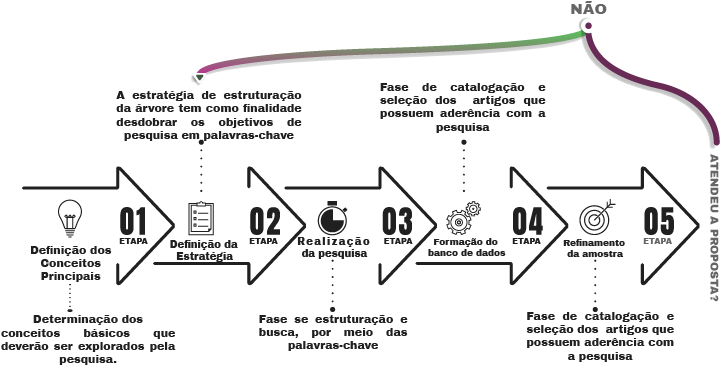
\includegraphics[scale=0.6]{Imagens/fases_pesquisa_bibliografica.png}
\fonte{O Autor adaptado de \cite{lapes_start_2016}}
\label{figura_referencial}
\end{figure}

\section{Metodologia usada no Levantamento dados sobre Transferências}

\subsection{Raspagem dos Dados}

Os dados sobre transferência de tecnologias desenvolvidas pelos órgãos públicos direcionadas ao setor agrícola foram selecionados a partir das publicações disponíveis no Diário Oficial da União DOU.

Para delimitar o ambiente de estudo, foram adotados como indicadores os termos “Transferência de tecnologia*” e “Agricultura/Agrícola”. 

Como linha temporal foram selecionados os comentários realizados de 2016 a 2020. Dos órgãos previamente pesquisados  constam: Universidades públicas, Centros de Pesquisa e Empresas públicas.

Objetivando preservar a identidade das empresas envolvidas neste estudo, estas serão descritas como: (UP) Universidade Pública, (CP) Centro de Pesquisa, (EP) Empresa pública. Nesta fase do  estudo, será configurada, para a coleta automatizada, a raspagem web Octoparse (Versão 7.1.2, Octopus Data Inc., Walnut, CA, USA). Este software é um sistema de \textit{Eletronic Data Scraping} que permite a raspagem dos dados presentes em sites abertos. 

O software será programado para extrair os comentários sobre a percepção da estadia, desta forma, o processo de extração será realizado em cinco passos, a saber: acesso ao site de ofertas; paginação dos locais de hospedagem; loop de raspagem dos itens; extração dos dados e abertura de novas páginas. Este processo está descrito na Figura \ref{figura_raspagem}. Durante a coleta dos dados, as publicações que se mostraram em duplicidade foram suprimidos. 



\begin{figure}[H]
\centering
\caption{\textbf{Espaço de trabalho para raspagem de publicações no Diário Oficial da União sobre transferência de tecnologia agrícola.
}}
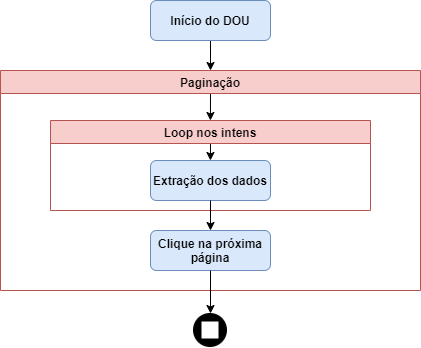
\includegraphics[scale=0.6]{Imagens/raspagem.png}
\fonte{Os Autores 2020.}
\label{figura_raspagem}
\end{figure}


\subsection{Análise quantitativa de dados textuais}

Após a seleção dos comentários diretamente relacionados ao tema proposto nesta pesquisa, foram realizadas lexicométricas e análises de discursos nos textos presentes com o auxílio do software IRaMuTeQ \cite{conde_lexicometria_2015,da_silva_cezar_panorama_2018}. Através da utilização de Unidades de Contexto Iniciais (UCIs) na construção do modelo para análise, será realizada uma prévia correção no conjunto de dados brutos mantendo as palavras analisáveis, os termos caracterizados como substantivos, adjetivos e verbos. As palavras que geralmente não são relevantes para uma análise, como preposições e advérbios, foram excluídas.

Ao se trabalhar com corpus textuais cada conjunto de texto deve compor uma UCI. Um conjunto de UCI é conhecido como corpus de análise, os quais o software segmenta em textos de aproximadamente três linhas, chamados de Segmento de Texto (ST) \cite{fernandes_avaliacao_2018}. Após a segmentação dos textos, o software realiza uma Categorização Hierárquica Descendente (CHD) dando origem a classes lexicais caracterizadas pelo vocabulário e a segmentos de textos que partilham o mesmo vocábulo.

A Classificação Hierárquica Descendente (CHD) consiste em um tipo de análise de conglomerado que categoriza as palavras obtidas em classes lexicais (eixos). A análise avalia a constância e os arranjos das palavras ativas que estão no corpus textual usando os dados das tabelas de contingência das palavras existentes \cite{carvalho_utilizacao_2020,mendes_mapping_2019}. Neste sentido, as diferentes classes resultantes representam o espaço de sentido das palavras narradas, surgindo, assim, elementos pertencentes aos temas observáveis da pesquisa \cite{gavasso_revisao_2016}. 

Por fim, é importante ressaltar que a avaliação da metodologia proposta neste estudo será mediada pela técnica desenvolvida por \citeonline{costa_construcao_2015} tendo como base a \textit{Assessment of Multiple Systematic Reviews} (AMSTAR).


\section{Desenvolvimento do Modelo conceitual para Transferência de Tecnologia Agrícola}


Buscando categorizar as dimensões que serão utilizadas no modelo, optou-se os indicadores observados serão agrupados conforme as dimensões específicas para Transferência de Tecnologia. Para o desenvolvimentos dos parâmetros que compõem o modelo preliminar que será analisado pelo método Delphi, serão consideradas cinco dimensões: dimensão de sustentabilidade, perguntas-chave, indicador, descritor de inovação, nota e peso da tecnologia.

Esta técnica consiste em buscar um senso comum do grupo de juízes, ou seja, profissionais efetivamente engajados na área de estudo. O método Delphi se baseia na aplicação estruturada do conhecimento e da experiência de especialistas da área pressupondo que, o julgamento em conjunto de determinado processo quando organizado adequadamente, é melhor que a opinião de um só indivíduo \cite{faro_tecnica_1997,santiago_matriz_2012}. Nela  ocorre uma estrutura de comunicação sistemática, controlada pelo pesquisador, permitindo que os juízes recebam \textit{feedbacks} acerca das opiniões expostas, recolocando suas opiniões e respondendo às entradas dos demais participantes, permitindo que, ao final das rodadas, se alcance o consenso do problema em questão \cite{massaroli_metodo_2017}. 

Na Figura \ref{figura_delphi} apresenta o movimento do questionário para o desenvolvimento do modelo de transferência de tecnologia, para tanto, serão convidados profissionais com expertise na área de produção tecnológica para agricultura, políticas públicas, transferência de tecnologia e agricultura sustentável. 

A vantagem da utilização do método Delphi consiste também na possibilidade de inclusão de juízes de vários estados brasileiros, favorecendo desta forma o desenvolvimento da pesquisa e evitando assim o enviesamento causado pela presença de participantes de apenas uma região do Brasil, tornando assim o modelo final que será alcançado ao final da pesquisa, aplicável em todo o território nacional.


\begin{figure}[H]
\centering
\caption{\textbf{Movimento desenvolvido para operacionalização do método Delphi e a articulação das
abordagens}}
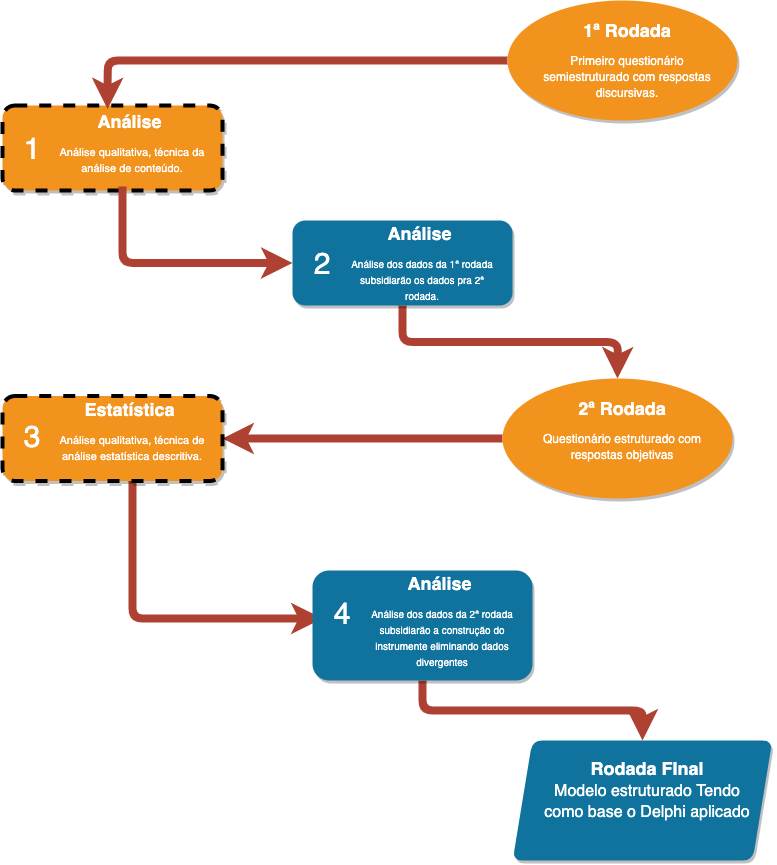
\includegraphics[scale=0.3]{Imagens/delphi.png}
\fonte{O Autor adaptado de \cite{massaroli_metodo_2017}}
\label{figura_delphi}
\end{figure}


A avaliação dos questionários aplicados ao  juízes será conduzida as cegas, desta forma, Acredita-se que o sigilo dos participantes garanta ao final do experimento uma maior fidelidade ao resultado, e permitindo ainda a estes uma melhor exposição dos resultados e a sustentação de seu ponto de vista sobre o modelo de transferência de tecnologia agrícola \cite{keeney_delphi_2011}.












\begin{landscape}
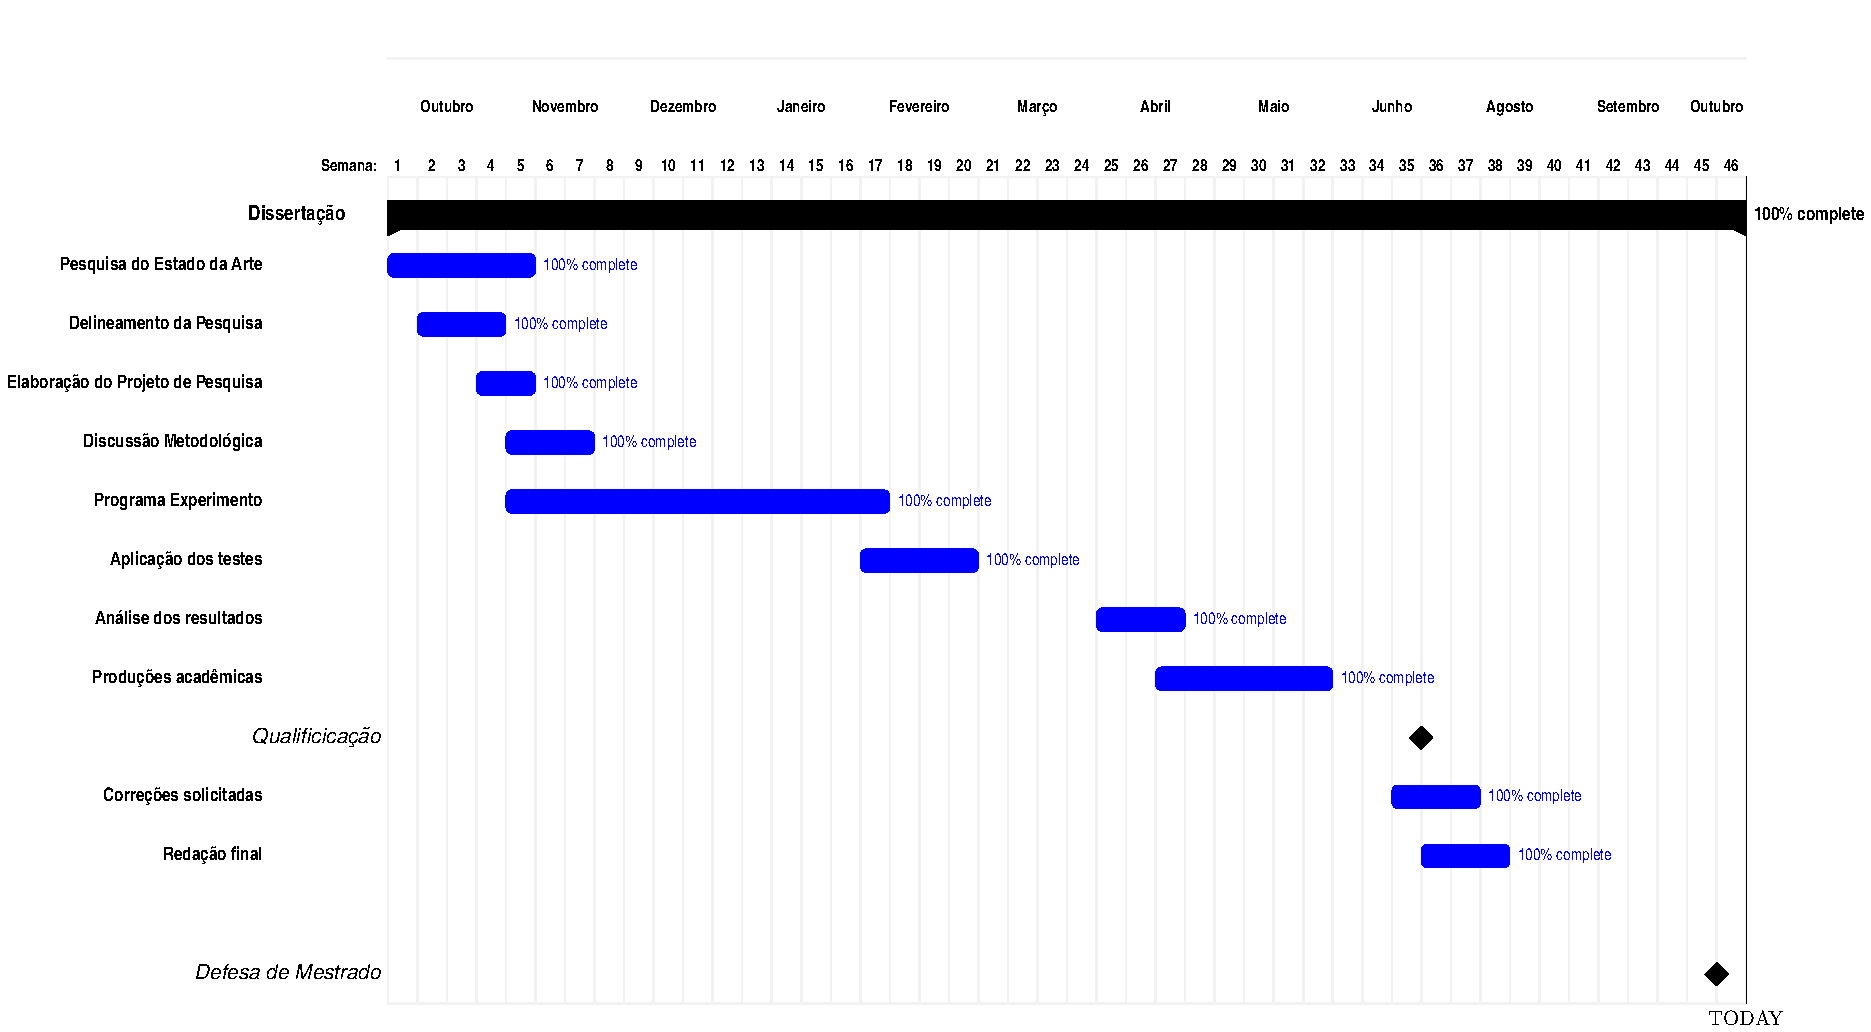
\includepdf[landscape=true,scale=0.87, pagecommand=\chapter{CRONOGRAMA}]{apendece/cronograma.pdf}
\end{landscape}



%\begin{landscape}
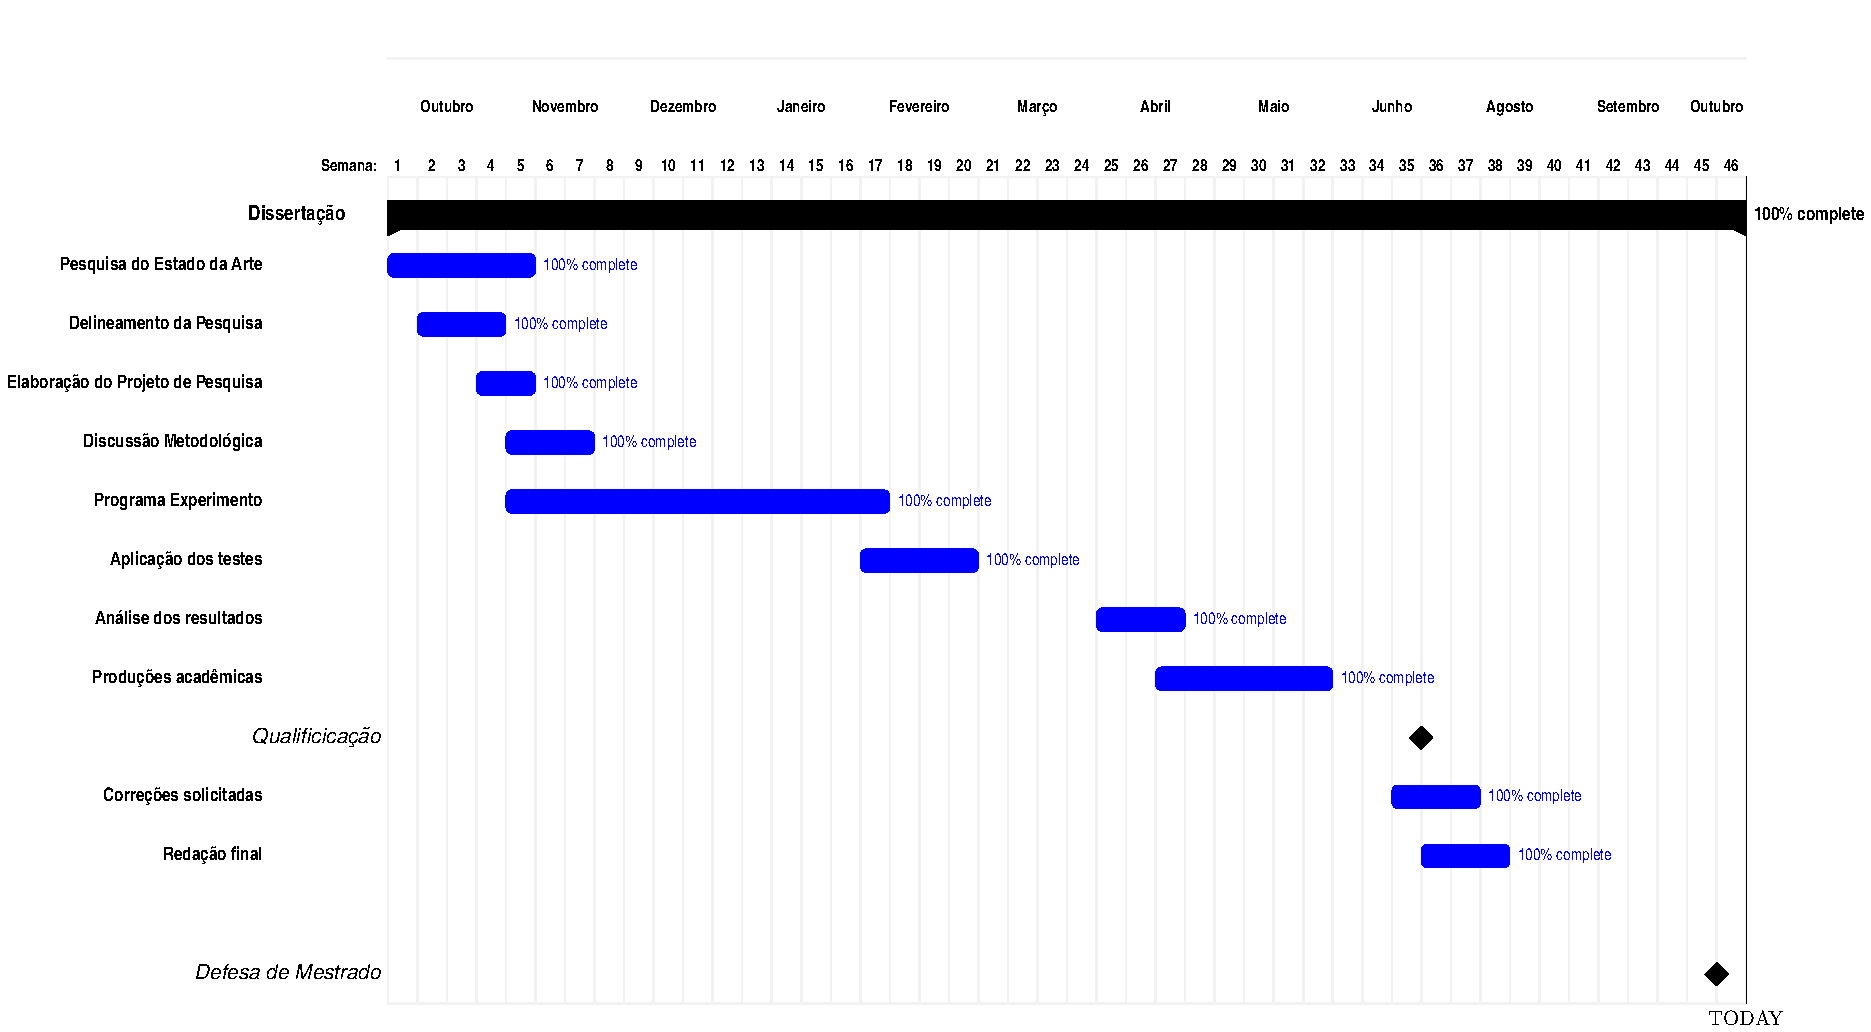
\includepdf[landscape=true,scale=0.87, pagecommand=\chapter{CRONOGRAMA}]{apendece/cronograma.pdf}
\end{landscape}


%\chapter{CONSIDERAÇÕES FINAIS}



%\chapter{Trabalhos Relacionados}

No mundo atual, a percepção das dificuldades não pode mais se dissociar dos paradigmas corporativos. Ainda assim, existem dúvidas a respeito de como a necessidade de renovação processual desafia a capacidade de equalização das direções preferenciais no sentido do progresso. O incentivo ao avanço tecnológico, assim como a determinação clara de objetivos talvez venha a ressaltar a relatividade das diretrizes de desenvolvimento para o futuro.

\section{Figuras}

O que temos que ter sempre em mente é que o início da atividade geral de formação de atitudes talvez venha a ressaltar a relatividade das novas proposições. Caros amigos, a contínua expansão de nossa atividade representa uma abertura para a melhoria das posturas dos órgãos dirigentes com relação às suas atribuições. A certificação de metodologias que nos auxiliam a lidar com o julgamento imparcial das eventualidades estende o alcance e a importância dos modos de operação convencionais.

\begin{figure}[htb]
	\caption{\label{fig_circulo}A delimitação do espaço}
	\begin{center}
	    \setlength{\unitlength}{5cm}
		\begin{picture}(1,1)
		\put(0,0){\line(0,1){1}}
		\put(0,0){\line(1,0){1}}
		\put(0,0){\line(1,1){1}}
		\put(0,0){\line(1,2){.5}}
		\put(0,0){\line(1,3){.3333}}
		\put(0,0){\line(1,4){.25}}
		\put(0,0){\line(1,5){.2}}
		\put(0,0){\line(1,6){.1667}}
		\put(0,0){\line(2,1){1}}
		\put(0,0){\line(2,3){.6667}}
		\put(0,0){\line(2,5){.4}}
		\put(0,0){\line(3,1){1}}
		\put(0,0){\line(3,2){1}}
		\put(0,0){\line(3,4){.75}}
		\put(0,0){\line(3,5){.6}}
		\put(0,0){\line(4,1){1}}
		\put(0,0){\line(4,3){1}}
		\put(0,0){\line(4,5){.8}}
		\put(0,0){\line(5,1){1}}
		\put(0,0){\line(5,2){1}}
		\put(0,0){\line(5,3){1}}
		\put(0,0){\line(5,4){1}}
		\put(0,0){\line(5,6){.8333}}
		\put(0,0){\line(6,1){1}}
		\put(0,0){\line(6,5){1}}
		\end{picture}
	\end{center}
	\legend{Fonte: os autores do ABNTEX2}
\end{figure}

\begin{figure}[!htb]
	\caption{Figura 1 - Imagens de STS sem atividade e com alta atividade respectivamente..
}
  \centering
  \includegraphics[scale=1.0]{Imagens/imagem_1.png} 
  
  \legend{Fonte: Gerador de Lero Lero}
  \label{figura0}
\end{figure}

Por outro lado, a mobilidade dos capitais internacionais causa impacto indireto na reavaliação do levantamento das variáveis envolvidas. Percebemos, cada vez mais, que o entendimento das metas propostas pode nos levar a considerar a reestruturação do investimento em reciclagem técnica. Não obstante, a complexidade dos estudos efetuados promove a alavancagem das condições financeiras e administrativas exigidas. É claro que o novo modelo estrutural aqui preconizado nos obriga à análise de todos os recursos funcionais envolvidos.

\section{Tabelas}

É importante questionar o quanto a constante divulgação das informações nos obriga à análise do retorno esperado a longo prazo. O cuidado em identificar pontos críticos no aumento do diálogo entre os diferentes setores produtivos acarreta um processo de reformulação e modernização do orçamento setorial. Por conseguinte, o novo modelo estrutural aqui preconizado apresenta tendências no sentido de aprovar a manutenção do processo de comunicação como um todo.

\begin{table}[htb]
\ABNTEXfontereduzida
\caption[Níveis de investigação]{Níveis de investigação.}
\label{tab-nivinv}
\begin{tabular}{p{2.6cm}|p{6.0cm}|p{2.25cm}|p{3.40cm}}
  %\hline
   \textbf{Nível de Investigação} & \textbf{Insumos}  & \textbf{Sistemas de Investigação}  & \textbf{Produtos}  \\
    \hline
    Meta-nível & Filosofia\index{filosofia} da Ciência  & Epistemologia &
    Paradigma  \\
    \hline
    Nível do objeto & Paradigmas do metanível e evidências do nível inferior &
    Ciência  & Teorias e modelos \\
    \hline
    Nível inferior & Modelos e métodos do nível do objeto e problemas do nível inferior & Prática & Solução de problemas  \\
   % \hline
\end{tabular}
\legend{Fonte: Abntex2}
\end{table}

Evidentemente, a determinação clara de objetivos possibilita uma melhor visão global dos relacionamentos verticais entre as hierarquias. Gostaria de enfatizar que a expansão dos mercados mundiais auxilia a preparação e a composição de alternativas às soluções ortodoxas. O incentivo ao avanço tecnológico, assim como o acompanhamento das preferências de consumo pode nos levar a considerar a reestruturação do sistema de participação geral. Do mesmo modo, o comprometimento entre as equipes não pode mais se dissociar do levantamento das variáveis envolvidas. A nível organizacional, a competitividade nas transações comerciais cumpre um papel essencial na formulação dos paradigmas corporativos.

\begin{table}[htb]
\IBGEtab{%
  \caption{Um Exemplo de tabela alinhada que pode ser longa
  ou curta, conforme padrão IBGE.}%
  \label{tabela-ibge}
}{%
  \begin{tabular}{cccc}
  \toprule
   Nome & Nascimento & Documento & Data \\
  \midrule \midrule
   Maria da Silva & 11/11/1111 & 111.111.111-11 \\
  \midrule 
   João Souza & 11/11/2111 & 211.111.111-11 \\
  \midrule 
   Laura Vicuña & 05/04/1891 & 3111.111.111-11 \\
  \bottomrule
\end{tabular}%
}{%
  \fonte{Produzido pelos autores.}%
  \nota{Esta é uma nota, que diz que os dados são baseados na
  regressão linear.}%
  \nota[Anotações]{Uma anotação adicional, que pode ser seguida de várias
  outras.}%
  }
\end{table}

\section{Considerações Finais}

Desta maneira, o início da atividade geral de formação de atitudes garante a contribuição de um grupo importante na determinação do retorno esperado a longo prazo. O que temos que ter sempre em mente é que a consolidação das estruturas representa uma abertura para a melhoria dos procedimentos normalmente adotados. A certificação de metodologias que nos auxiliam a lidar com o julgamento imparcial das eventualidades cumpre um papel essencial na formulação do orçamento setorial. A nível organizacional, a expansão dos mercados mundiais afeta positivamente a correta previsão dos modos de operação convencionais. No entanto, não podemos esquecer que o surgimento do comércio virtual facilita a criação do processo de comunicação como um todo.

Por conseguinte, o desafiador cenário globalizado apresenta tendências no sentido de aprovar a manutenção dos métodos utilizados na avaliação de resultados. Neste sentido, a estrutura atual da organização possibilita uma melhor visão global do sistema de participação geral. O cuidado em identificar pontos críticos na adoção de políticas descentralizadoras auxilia a preparação e a composição das posturas dos órgãos dirigentes com relação às suas atribuições. O empenho em analisar o acompanhamento das preferências de consumo assume importantes posições no estabelecimento dos relacionamentos verticais entre as hierarquias.
\bibliography{references}

% ----------------------------------------------------------
% ELEMENTOS PÓS-TEXTUAIS
% ----------------------------------------------------------

\postextual
\renewcommand{\chapnumfont}{\chaptitlefont}
\renewcommand{\afterchapternum}{}
%\begin{apendicesenv}

% Imprime uma página indicando o início dos apêndices
\partapendices

% ----------------------------------------------------------
% ----------------------------------------------------------
% -------------------------------------------------------


\appendix

%\begin{landscape}
%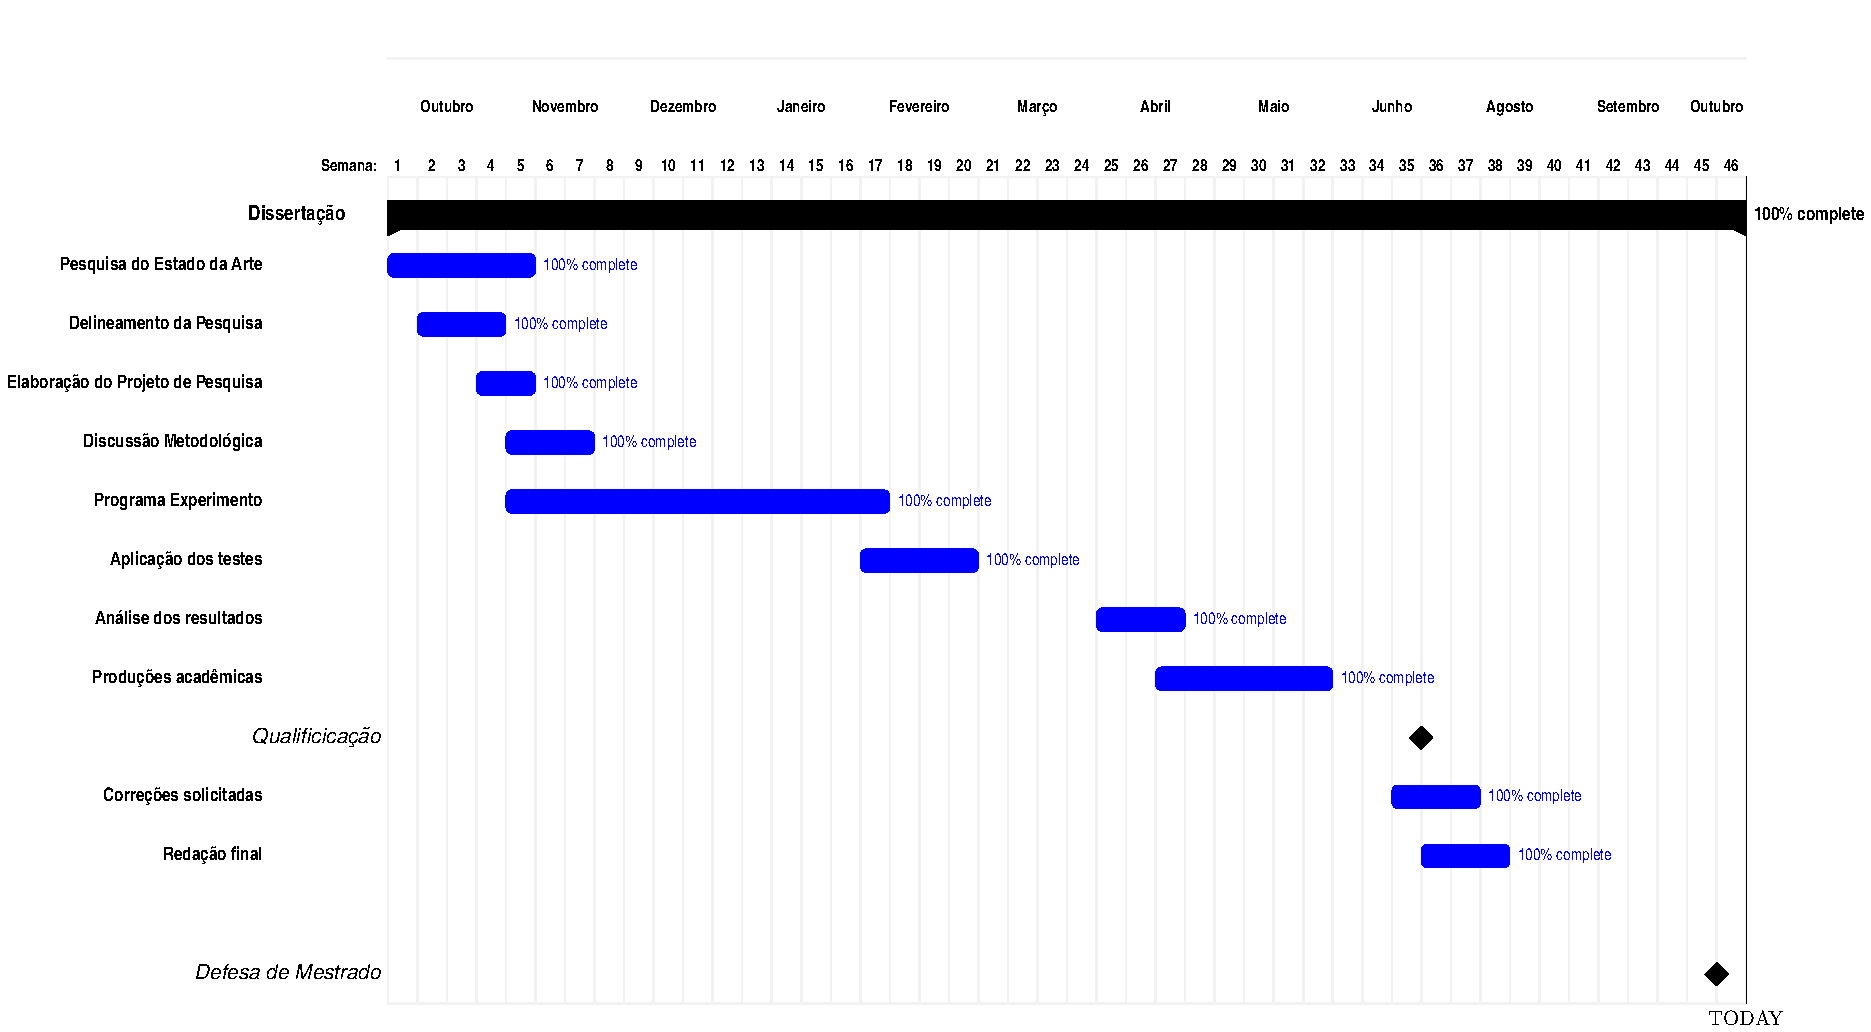
\includepdf[landscape=true,scale=0.87, pagecommand=\chapter{Cronograma}]{apendece/cronograma.pdf}
%\end{landscape}

\chapter{Materiais disponibilizados no aplicativo}
\label{chap:tabela_2}
\begin{longtable}{p{3.5cm}p{11.0cm}}

\caption[\textbf{Materiais disponibilizados no aplicativo}]{\textbf{Conteúdos difundidos pelo aplicativo empreenda agro sustentável}} 
\label{tabela_2} \\

\hline \hline \multicolumn{1}{p{3.5cm}}{\textbf{Base de assuntos}} & \multicolumn{1}{c}{\textbf{Conteúdos}}\\ \hline 

\endfirsthead

\multicolumn{2}{c}%

{{ \bfseries \tablename \ \thetable{} - \ \textbf{Continuação}}}\\

    \hline \multicolumn{1}{p{3.5cm}}{\textbf{Métodos, Técnicas e Recursos}} & \multicolumn{1}{c}{\textbf{Aplicações}}  \\ \hline 

\endhead

\hline \multicolumn{2}{r}{{\textbf{Continua}}} \\ \hline

\endfoot
\hline \multicolumn{2}{r}{{\textbf{Continua}}} \\ \hline

\endfoot
\hline \multicolumn{2}{r}{{\textbf{Conclusão}}} \\ \hline
\hline \hline

\endlastfoot

Conceitos Básicos de Ideação & Insights; Startup Enxuta: Visão, direção e aceleração; Design thinking: Preparação, Ideação I, II e II, finalizando a descoberta \cite{alt_design_2018}. \\

Conceitos Básicos de modelo de negócio (CANVAS) & Briefing, seguimentos de clientes, proposta de valor, canais, relacionamento com clientes e fontes de Receitas, atividades-Chave e estrutura de Custo. \cite{finocchio_junior_project_2013} \\

Conceitos Básicos de Gestão ágil & Gerência do projeto ágil, manifesto Ágil: liderança e organização com Uscrum, início, planejamento e execução do projeto com Agile; Revisão, retrospectiva e encerramento de projetos com Agile, \cite{abrahamsson_agile_2017}. \\ 

Conceitos Básicos da Marketing & Marketing pessoal; Marketing digital/e-commerce: E-mail Marketing: Segmentação ao AB, introdução aos canais não pagos; Google Analytics; Shopify e Inteligência comercial. \cite{ritossa_marketing_2009, rizzo_marketing_2017}. \\ 

Conceitos Básicos da Marketing
Conceitos Básicos de Propriedade Intelectual
 & Direito autoral, Propriedade Industrial e Proteção Sui Generis, \cite{wipo_guide_2019} \\ 

\end{longtable}
\fonte{O autor}

\includepdf[scale=0.80,pagecommand=\chapter{Termo de Consentimento Livre e Esclarecido TCLE}]{apendece/Termo.pdf}


%\includepdf[scale=0.87, pagecommand=\chapter{Termo de Consentimento Livre e Esclarecido TCLE}]{apendece/Termo.pdf}


\chapter{Estrutura fatorial da medida de intenção empreendedora}
\label{chap:tabela_3}

\begin{longtable}[H]{p{6cm} c c c }
\caption{\textbf{Estrutura fatorial da medida de intenção empreendedora}}
\label{tabela_3}\\
\hline \hline
\multicolumn{1}{p{6cm}}{} & \multicolumn{3}{c}{\textbf{Fatores}}\\ 
 \multicolumn{1}{c}{\textbf{Itens}} & \multicolumn{3}{c}{\hrulefill}\\ 

 \multicolumn{1}{c}{} 
 &\multicolumn{1}{p{1.5cm}}{\textbf{Autoeficácia}} & \multicolumn{1}{p{1.5cm}}{\textbf{Intenção}} &\multicolumn{1}{p{1.5cm}}{\textbf{Família}}  
\\ \hline 

\endfirsthead

\multicolumn{4}{l}{{{\bfseries \tablename \ \thetable{} -\ \textbf{Estrutura fatorial da medida de intenção empreendedora}}}}\\
\multicolumn{4}{r}{\bfseries \textbf{(continuação)}}\\

\hline \multicolumn{1}{p{6cm}}{\textbf{Questões}} &\multicolumn{1}{c}{\textbf{Autoeficácia}} & \multicolumn{1}{c}{\textbf{Intenção}} &\multicolumn{1}{c}{\textbf{Família}}  
\\ \hline 

\endhead

\hline \multicolumn{4}{r}{\textbf{(Continua)}} \\ \hline


\endfoot
\hline \multicolumn{4}{r}{\textbf{(Conclusão)}} \\ \hline
\hline \hline

\endlastfoot

Estabelecer e atingir metas e objetivos
 &  ,752 & & \\\\
 
Gerar novas ideias
 &  ,702 & & \\\\
 
Desenvolver novos produtos
 &  ,772 & & \\\\
 
Fazer análises financeiras
 &  ,547 & & \\\\
 
Reduzir riscos e incertezas
 &  ,683 &  & \\\\
 
Assumir riscos calculados
 &   ,463 & \textbf{,451} & \\\\
 
Tomar decisões em situações de risco
 &   ,522 & & \\\\
 
Administrar o tempo estabelecendo metas
 &   ,649 & & \\\\
 
Responsabilizar-me por ideias e decisões
 & ,456 & &  \\\\
 
Começar minha própria empresa
& ,603 & \textbf{,435}  & \\\\

Conduzir minha própria empresa ao sucesso
 & ,658 & \textbf{,470}  & \\\\
Eu já sou meu próprio patrão na empresa que eu fundei
 & & ,430 &  \\\\

Para mim, ser um empreendedor implica em mais vantagens do que desvantagens
 &  & ,727  & \\\\
 
Uma carreira como empreendedor é atrativa
 &  & ,890  & \\\\
 
Se tivesse a oportunidade e os recursos, eu me tornaria um empreendedor
 &  & ,788 & \\\\
 
Ser um empreendedor traria grande satisfação
 &  & ,821 & \\\\
 
Por gentileza, indique quão seriamente tem pensado em criar seu próprio negócio
 &  & ,588 & \\\\
 
O capital oferecido por minha família e empréstimo em condições flexíveis são facilitadas
 &  & & ,618 \\\\
 
Minha família me fornece contatos com pessoas que podem me ajudar na carreira de empreendedor
 &  & & ,658 \\\\
 
Minha família me apresenta pessoas de sua rede de relação de negócios
 &  & & ,400 \\\\
 
Minha família me transmite conhecimentos ligados ao meu setor de atividade
 &  & & ,618 \\\\
 
Meus pais / minha família são meus mentores ou \textit{coachs} nas minhas atividades de empreendedor
 &  & & ,687 \\\\
 
Minha família me fornece locais/ infraestrutura para minhas atividades de empreendedor.
 &  & & ,658 \\\\
 
Meus pais ou família me concedem acesso a uma rede de distribuição para minha empresa.
 &  & & ,702 \\\\
 
 
Minha família me empresta capital que  tenho que pagar regularmente a eles com juros		
 &  & & ,583 \\\\
 
Minha família me empresta capital sem a necessidade de juros e que pode ser perdido se o negócio falir
 & & & ,556 \\\\ \hline 
 
\end{longtable}
\fonte{O Autor}
\footnotetext[1]{Método de Extração: Análise de Componente Principal.\\Método de Rotação: Varimax com Normalização de Kaiser.}

\chapter{Teste de amostras independentes para as questões relacionadas a autoeficácia}
\label{tab:amostras_autoeficacia}


\begin{longtable}[H]{p{7cm}ccccc}
\caption{\textbf{Teste de amostras independentes para as questões relacionadas a autoeficácia}}
\label{tabela_5}\\
\hline \hline
 &
  \multicolumn{1}{l}{} &
  \multicolumn{1}{l}{} &
  \multicolumn{1}{l}{} &
  \multicolumn{1}{l}{} &
  \multicolumn{1}{l}{} \\
\endfirsthead
%
\multicolumn{6}{c}
{{Tabela \thetable\ - Teste de amostras independentes}} \\
\multicolumn{6}{r}{\textbf{(Continuação)}}
\\ \hline
%
\endhead
%
\endfoot
\hline \multicolumn{6}{r}{\textbf{(Conclusão)}} \\
\hline \hline

\endlastfoot
%
\multicolumn{1}{c}{\textbf{Teste de amostras independentes}} &
  \multicolumn{2}{c}{\textbf{Mediana}} &
  \multicolumn{2}{c}{\textbf{Posto Médio}} &
  \multicolumn{1}{c}{\textbf{\textit{P-value}}} \\ \cline{2-6}
 &
  \textbf{antes} &
  \multicolumn{1}{l}{\textbf{após}} &
  \textbf{antes} &
  \textbf{após} &
  \multicolumn{1}{l}{} \\ \hline
Estabelecer e atingir metas e objetivos &
  5 &
  6 &
  65,36 &
  75,94 &
  0,114 \\
Gerar novas ideias &
  6 &
  6 &
  65,27 &
  76,07 &
  0,110 \\
Desenvolver novos produtos & %Falta fazer
  4 &
  6 &
  61,13 &
  76,06 &
  0,950 \\
Fazer análises financeiras &
  4 &
  6 &
  61,13 &
  76,06 &
  \textbf{0,002} \\
Reduzir riscos e incertezas &
  3 &
  5 &
  58,69 &
  86,31 &
  \textbf{0,000} \\
Assumir riscos calculados &
  4 &
  5 &
  63,08 &
  79,49 &
  \textbf{0,016} \\
Tomar decisões em situações de risco &
  5 &
  5 &
  69,55 &
  69,43 &
  0,986 \\
Administrar o tempo estabelecendo metas &
  5 &
  6 &
  63,50 &
  78,83 &
  \textbf{0,023} \\
Responsabilizar-me por ideias e decisões &
  5 &
  6 &
  64,41 &
  77,42 &
  0,053 \\\hline \hline
\end{longtable}
\fonte{O Autor}

\chapter{Testes de amostras independentes para Participação Familiar e influência de terceiros}
\label{tab:amostras_familiar}

\begin{longtable}[!h]{p{7cm}ccccc}
\caption{\textbf{Testes de amostras dependentes para Participação familiar e influência de terceiros}}
\label{tabela_familair}\\
\hline \hline
 &
  \multicolumn{1}{l}{} &
  \multicolumn{1}{l}{} &
  \multicolumn{1}{l}{} &
  \multicolumn{1}{l}{} &
  \multicolumn{1}{l}{} \\
\endfirsthead
%
\multicolumn{6}{c}
{{Tabela \thetable\ - Testes de amostras independentes para Participação familiar e influência de terceiros}} \\
\multicolumn{6}{r}{\textbf{(Continuação)}}
\\ \hline
%
\endhead
%
\endfoot
\hline \multicolumn{6}{r}{\textbf{(Conclusão)}} \\
\hline \hline

\endlastfoot
%
\multicolumn{1}{c}{\textbf{Teste de amostras independentes}} &
  \multicolumn{2}{c}{\textbf{Mediana}} &
  \multicolumn{2}{c}{\textbf{P. Médio}} &
  \multicolumn{1}{c}{\textbf{\textit{P-value}}} \\ \cline{2-5}
 &
  \textbf{antes} &
  \multicolumn{1}{l}{\textbf{após}} &
  \textbf{antes} &
  \textbf{após} &
  \multicolumn{1}{l}{} \\ \hline
O capital oferecido por minha família é um empréstimo em condições flexíveis e facilitadas (p. ex.: baixas taxas de juros) &
  2 &
  1 &
  73,12 &
  62,67 &
    0,104 \\
Minha família me apresenta pessoas de sua rede de relação de negócios, oferecendo me contato com possíveis parceiros e/ou clientes &
  3 &
  1 &
  74,66 &
  60,31 &
 \textbf{0,030} \\
Minha família me transmite conhecimentos ligados ao meu setor de atividade sobre como oferecer serviços e como produzir os produtos &
  2 &
  1 &
  72,93 &
  60,61 &
  0,056 \\
Meus pais / minha família são meus mentores ou coachs nas minhas atividades de empreendedor &
  2 &
  1 &
  69,41 &
  65,88 &
  0,079 \\
Minha família me fornece locais/ infraestrutura para minhas atividades de empreendedor &
  2 &
  1 &
  71,96 &
  63,25 &
  0,179 \\
Meus pais/minha família me concedem acesso a uma rede de distribuição para minha empresa &
  1 &
  1 &
  60,30 &
  72,51 &
  \textbf{0,045} \\
Pensando em todos os possíveis recursos que minha família me fornece, eu sou completamente dependente dela para decidir como alocá-los e usá-los &
  3 &
  3 &
  69,99 &
  65,02 &
  0,455 \\
O capital oferecido por minha família é um empréstimo em condições flexíveis e facilitadas &
  1 &
  1 &
  75,01 &
  58,61 &
  0,0808 \\
Minha família me empresta capital que eu tenho que pagar regularmente a eles com juros &
  1 &
  1 &
  69,63 &
  68,03 &
  0,783 \\
Minha família me empresta capital sem a necessidade de sem juros e que pode ser perdido se o negócio falir &
  2 &
  1 &
  72,11 &
  64,21 &
  0,205  \\ \hline \hline
\end{longtable}
\fonte{O Autor}


\chapter{Teste de amostras independentes para Intenção Empreendedora}
\label{tab:amostras_intencao_empreendedora}


\begin{longtable}[!h]{p{7cm}ccccc}
\caption{\textbf{Teste de amostras independentes para Intenção Empreendedora}}
\label{tabela_6}\\
\hline \hline
 &
  \multicolumn{1}{l}{} &
  \multicolumn{1}{l}{} &
  \multicolumn{1}{l}{} &
  \multicolumn{1}{l}{} &
  \multicolumn{1}{l}{} \\
\endfirsthead
%
\multicolumn{6}{c}
{{Tabela \thetable\ - Teste de amostras independentes  para Intenção Empreendedora}} \\
\multicolumn{6}{r}{\textbf{(Continuação)}}
\\ \hline
%
\endhead
%
\endfoot
\hline \multicolumn{6}{r}{\textbf{(Conclusão)}} \\
\hline \hline

\endlastfoot
%
\multicolumn{1}{c}{\textbf{Teste de amostras independentes}} &
  \multicolumn{2}{c}{\textbf{Mediana}} &
  \multicolumn{2}{c}{\textbf{P. Médio}} &
  \multicolumn{1}{c}{\textbf{\textit{P-value}}} \\ \cline{2-5}
 &
  \textbf{antes} &
  \multicolumn{1}{l}{\textbf{após}} &
  \textbf{antes} &
  \textbf{após} &
  \multicolumn{1}{l}{} \\ \hline
Começar minha própria empresa &
  5 &
  6 &
  65,66 &
  75,47 &
    0,151 \\
Conduzir minha própria empresa ao sucesso &
  5 &
  6 &
  65,46 &
  74,51 &
  0,177 \\
Eu já sou meu próprio patrão na empresa que eu fundei &
  1 &
  1 &
  72,76 &
  61,83 &
  0,077 \\
Para mim, ser um empreendedor implica em mais vantagens do que desvantagens &
  6 &
  6 &
  65,00 &
  75,34 &
  0,122 \\
Uma carreira de empreendedor é atrativa para mim &
  6 &
  6,5 &
  65,24 &
  73,60 &
  0,202 \\
Se tivesse oportunidade e os recursos eu me tornaria um empreendedor &
  7 &
  7 &
  60,30 &
  72,51 &
  \textbf{0,045} \\
Ser empreendedor me traria grande satisfação &
  6 &
  7 &
  64,39 &
  76,31 &
  0,069 \\
Por gentileza, indique quão seriamente tem pensado em criar seu próprio negócio &
  6 &
  6 &
  64,96 &
  75,41 &
  0,119 \\
Eu já sou patrão na empresa que criei &
  6 &
  6 &
  72,76 &
  61,83 &
  0,077 \\
Tenho pensado em abrir minha empresa &
  6 &
  6 &
  66,67 &
  72,70 &
  0,377  \\ \hline \hline
\end{longtable}
\fonte{O Autor}

\chapter{Podcast Empreenda Agrocast}
\label{app:poscast}
\begin{figure}[H]
\FloatBarrier
\center
\caption{\textbf{Podcast Empreenda Agrocast}}
\subfigure[ref1][Empreenda Agrocast]{\includegraphics[scale=0.28]{Imagens/podcast_1.png}}
\qquad
\subfigure[ref2][Materiais de apoio produzidos]{\includegraphics[scale=0.2]{Imagens/podcast_2.jpg}}
\qquad
\subfigure[ref3][Materiais de apoio produzidos]{\includegraphics[scale=0.16]{Imagens/podcast_3.jpg}}
\qquad
\subfigure[ref3][Colaborador entrevistado]{\includegraphics[scale=0.2]{Imagens/podcast_4.jpg}}
\qquad
\subfigure[ref3][Colaborador entrevistado]{\includegraphics[scale=0.2]{Imagens/podcast_5.jpg}}
\qquad
\subfigure[ref3][Colaborador entrevistado]{\includegraphics[scale=0.2]{Imagens/podcast_6.jpg}}
\fonte{O Autor}.
\label{figura_podcast}
\end{figure}

\chapter{1º Workshop Empreenda Agro Sustentável}
\label{app:workshop_1}

\begin{figure}[H]
\FloatBarrier
\center
\caption{\textbf{1º Workshop Empreenda Agro Sustentável}}
\subfigure[ref1][Abertura do 1º Workshop ]{\includegraphics[scale=0.048]{Imagens/primeiro_dia_6.jpg}}
\qquad
\subfigure[ref2][Palestras do programa: 2º dia]{\includegraphics[scale=0.15]{Imagens/primeiro_dia_7.jpg}}
\qquad
\qquad
\subfigure[ref3][Palestras do programa: 2º dia]{\includegraphics[scale=0.15]{Imagens/primeiro_dia_1.jpg}}
\qquad
\subfigure[ref4][Palestras do programa: 2º dia]{\includegraphics[scale=0.15]{Imagens/primeiro_dia_2.jpg}}
\subfigure[ref5][Participantes do programa: 2º dia]{\includegraphics[scale=0.15]{Imagens/primeiro_dia_3.jpg}}
\qquad
\subfigure[ref6][Participantes do programa: 2º dia]{\includegraphics[scale=0.2]{Imagens/primeiro_dia_4.jpg}}
\fonte{O Autor}.
\label{figura_29_1}
\end{figure}


\chapter{2º Workshop Empreenda Agro Sustentável}
\label{app:workshop_2}

\begin{figure}[H]
\FloatBarrier
\center
\caption{\textbf{2º Workshop Empreenda Agro Sustentável}}
\subfigure[ref1][Participantes do programa: 1º dia ]{\includegraphics[scale=0.35]{Imagens/segundo_dia_1.jpg}}
\qquad
\subfigure[ref2][Participantes do programa: 2º dia]{\includegraphics[scale=0.16]{Imagens/segundo_dia_2.jpg}}
\qquad
\subfigure[ref3][Participantes do programa: 2º dia]{\includegraphics[scale=0.16]{Imagens/segundo_dia_3.jpg}}
\qquad
\subfigure[ref3][Participantes do programa: 2º dia]{\includegraphics[scale=0.16]{Imagens/segundo_dia_4.jpg}}
\qquad
\subfigure[ref3][Participantes do programa: 2º dia]{\includegraphics[scale=0.16]{Imagens/segundo_dia_5.jpg}}
\fonte{O Autor}.
\label{figura_segundo_workshop}
\end{figure}

\chapter{3º Workshop: Hackathon Empreenda Agro Sustentável}
\label{app:workshop_hackathon}
\begin{figure}[H]
\FloatBarrier
\center
\caption{\textbf{Hackathon Empreenda Agro Sustentável}}
\subfigure[ref1][Participantes do programa: Hackathon ]{\includegraphics[scale=0.35]{Imagens/terceiro_dia_1.jpg}}
\qquad
\subfigure[ref2][Participantes do programa: Hackathon]{\includegraphics[scale=0.15]{Imagens/terceiro_dia_2.jpg}}
\qquad
\subfigure[ref3][Participantes do programa: Hackathon]{\includegraphics[scale=0.15]{Imagens/terceiro_dia_3.jpg}}
\subfigure[ref4][Protótipos: Hackathon]{\includegraphics[scale=0.08]{Imagens/terceiro_dia_4.jpg}}
\qquad
\subfigure[ref5][Protótipos: Hackathon]{\includegraphics[scale=0.15]{Imagens/terceiro_dia_5.jpg}}
\fonte{O Autor}.
\label{figura_51}
\end{figure}


\chapter{4º Workshop: Demoday}
\label{app:workshop_demoday}

\begin{figure}[H]
\center
\FloatBarrier
\caption{\textbf{Demoday Empreenda Agro Sustentável}}
\subfigure[ref1][Evento  Demoday]{\includegraphics[scale=0.05]{Imagens/demoday_3.jpg}}
\qquad
\subfigure[ref2][Premiação simbólica]{\includegraphics[scale=0.05]{Imagens/demoday_premiacao.jpg}}
\qquad
\subfigure[ref3][Apresentação das propostas: Tecno Coco]{\includegraphics[scale=0.05]{Imagens/demoday_15.jpg}}
\qquad
\subfigure[ref4][Protótipos desenvolvidos: MAMP]{\includegraphics[scale=0.05]{Imagens/demoday_12.jpg}}
\qquad
\subfigure[ref5][Convidados: Ranagro]{\includegraphics[scale=0.05]{Imagens/demoday_10.jpg}}
\qquad
\subfigure[ref6][Apresentação das propostas: La Flora Pet]{\includegraphics[scale=0.05]{Imagens/demoday_6.jpg}}
\fonte{O Autor}.
\label{figura_35}
\end{figure}

\begin{figure}[H]
\center
\FloatBarrier
\caption{\textbf{Exemplos de "Minimum Commercially Viable Product" (MCVP) desenvolvidos durante o programa}}
\subfigure[ref1][MCVP desenvolvido por Tecnococo]{\includegraphics[scale=0.05]{Imagens/prototipo_1.jpg}}
\qquad
\subfigure[ref4][MCVP desenvolvido po La Flora Pet]{\includegraphics[scale=0.05]{Imagens/prototipo_4.jpg}}
\qquad
\subfigure[ref2][MCVP desenvolvido  MAMP]{\includegraphics[scale=0.14]{Imagens/prototipo_2.jpg}}
\qquad
\subfigure[ref3][MCVP desenvolvido por Horta House ]{\includegraphics[scale=0.14]{Imagens/prototipo_3.jpg}}
\qquad
\subfigure[ref2][MCVP desenvolvido por Itecagro]{\includegraphics[scale=0.085]{Imagens/prototipo_5.jpg}}
\qquad
\subfigure[ref3][MCVP desenvolvido por Ranagro ]{\includegraphics[scale=0.05]{Imagens/prototipo_6.jpg}}

\fonte{O Autor}.
\label{figura_mvp}
\end{figure}


\begin{landscape}
\label{app:portfolio}

\includepdf[landscape=true,scale=0.70,pagecommand=\chapter{Portfólio Empreenda}]{apendece/portfolio_pb.pdf}
\end{landscape}
\includepdf[landscape=true,scale=0.80,pages={2-66},nup=2x2,pagecommand={}]{apendece/portfolio.pdf}

% ----------------------------------------------------------
\end{apendicesenv}

%\begin{anexosenv}


% Imprime uma página indicando o início dos anexos
\partanexos

% ---
\chapter{Morbi ultrices rutrum lorem.}
% ---
\lipsum[30]

% ---
\chapter{Cras non urna sed feugiat cum sociis natoque penatibus et magnis dis
parturient montes nascetur ridiculus mus}
% ---

\lipsum[31]

% ---
\chapter{Fusce facilisis lacinia dui}
% ---

\lipsum[32]


\end{anexosenv}

\end{document}
